% ch04-ml.tex -- Linear models and regularisation
\chapter{Linear models and regularisation}\label{ch:linear}

The linear model is where machine learning starts paying rent on its linear
algebra. One line of closed-form mathematics --- $\boldsymbol\theta =
(X^TX)^{-1}X^T\mathbf{y}$ --- delivers a fitted model, and everything in this
chapter is a variation on that theme: add a penalty and you get ridge and
lasso, wrap the score in a sigmoid and you get logistic regression, bend the
input with a feature map and you get polynomial regression. The recurring
question is the one Chapter 3 trained you to ask: not ``does it fit?'' but
``does it generalise, and what did the fit cost?'' Regularisation is the
answer engineered directly into the objective: accept a little bias on
purpose, in exchange for a lot less variance.\index{regularisation} Below we
derive every model used, implement two of them from scratch, and read
coefficient paths the way a senior engineer reads a flame graph.

% from-zero:begin
\begin{rulebox}[Before you start]
Chapter~3 and \textbf{Book~3, Chapter~8} (least squares). \emph{Recap:} the best-fit line minimises the sum of squared errors, and the normal equations $X^{\mathsf T}X\mathbf w=X^{\mathsf T}\mathbf y$ give the answer in one step.
\end{rulebox}
\begin{wins}[After this chapter you can]
\begin{itemize}
\item fit linear regression and read its coefficients;
\item use ridge and lasso to fight overfitting and say how they differ;
\item fit logistic regression and softmax for classification;
\item bend a linear model with a feature map, and explain the kernel trick in one paragraph.
\end{itemize}
\end{wins}
\begin{principle}[How to think about this]
A linear model is the simplest honest guess: the output is a weighted sum of the inputs. Training chooses the weights; regularisation says ``prefer small weights unless the data insist,'' which fights overfitting. If a straight line is not enough, bend the inputs (feature maps) instead of abandoning the line.
\end{principle}
% from-zero:end

\section{Least squares: the normal equations}\label{sec:ols}

\begin{definition}[Ordinary least squares]\index{least squares}
Given $X \in \mathbb{R}^{n\times d}$ (rows are samples, per Chapter 1) and
targets $\mathbf{y} \in \mathbb{R}^n$, the least-squares fit is
\[
\hat{\boldsymbol\theta} = \arg\min_{\boldsymbol\theta}
\|X\boldsymbol\theta - \mathbf{y}\|_2^2
= (X^TX)^{-1}X^T\mathbf{y},
\]
which exists uniquely when $X^TX$ is invertible --- i.e.\ $X$ has full
column rank.
\end{definition}

The derivation is one line of calculus (set $\nabla_{\boldsymbol\theta}
\|X\boldsymbol\theta - \mathbf{y}\|^2 = 0$) and one geometric fact: the
residual is orthogonal to the column space. The implementation is one line
of NumPy --- and you should call \texttt{solve}, never form the inverse.

\lstinputlisting[language=Python,caption={\texttt{code/ch04/linreg\_scratch.py}: OLS, the ridge path, and the singular-$X^TX$ rescue --- all closed-form.},label={lst:linreg}]{code/ch04/linreg_scratch.py}

\lstinputlisting[numbers=none]{code/ch04/linreg_scratch.out.txt}

\begin{example}[WE 4.1 --- When $X^TX$ is singular]\label{ex:singular}
Strategy: break the rank assumption deliberately and watch what the
coefficients do.\par
\begin{solution}
Listing~\ref{lst:linreg} appends a duplicate column ($x_{d+1} = 2x_3$) so
$X^TX$ is rank-deficient. OLS returns $\|\boldsymbol\theta\| \approx
7.9\times10^{17}$: infinitely many solutions exist and the solver picks a
catastrophic one --- huge cancelling coefficients that happen to fit.
Ridge with $\lambda{=}1$ on the same broken design returns
$\|\boldsymbol\theta\| = 478$: the penalty picks the \emph{small-norm}
solution from the infinite family. This is ridge's original job (it was
invented to solve unsolvable problems) --- regularisation here is not
preference, it is selection.
\end{solution}
\end{example}

\section{Ridge: shrink the coefficients}\label{sec:ridge}

\begin{definition}[Ridge regression]\index{ridge}
\[
\hat{\boldsymbol\theta}_{\text{ridge}} =
\arg\min_{\boldsymbol\theta}\;
\|X\boldsymbol\theta - \mathbf{y}\|_2^2 +
\lambda\|\boldsymbol\theta\|_2^2
= (X^TX + \lambda I)^{-1}X^T\mathbf{y}.
\]
The penalty applies to coefficients only --- the intercept is left
unpenalised (standardise first, or the scale of $\mathbf{x}$ decides the
shrinkage for you).
\end{definition}

$\lambda$ is the bias--variance dial of Chapter 3 made literal:
$\lambda{=}0$ is OLS (maximum variance), $\lambda\to\infty$ pins every
coefficient at zero (maximum bias). The train MSE climbs monotonically in
$\lambda$ while the test MSE traces the familiar U --- read it in
Figure~\ref{fig:ucurve} and in Listing~\ref{lst:linreg}'s table:
$2966 \to 2861$ near $\lambda \approx 0.1$, then $4246$ by $\lambda{=}10$.

\begin{figure}[ht]\centering
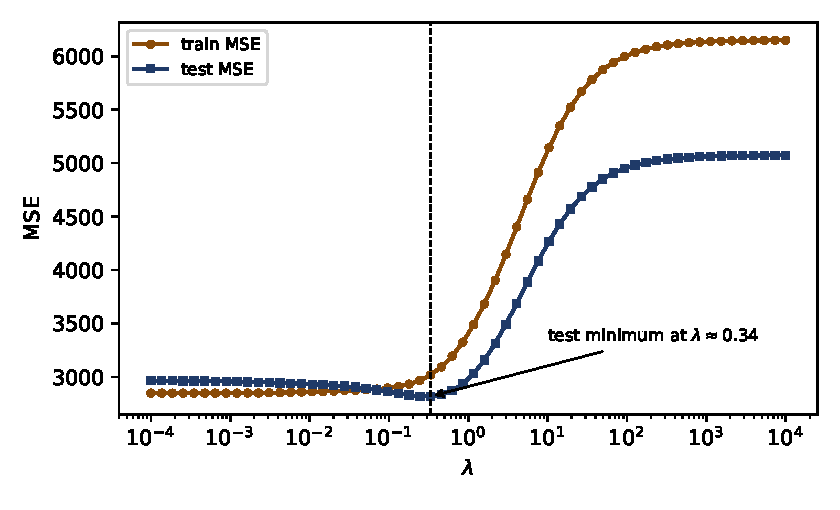
\includegraphics[width=0.72\linewidth]{figures/ch04/lambda_ucurve.pdf}
\caption{Train vs test MSE against $\lambda$ on \texttt{diabetes}
(\texttt{figures/fig\_ch04\_lambda\_ucurve.py}). Train error rises
monotonically; test error bottoms at $\lambda \approx 0.2$--$0.3$ and
climbs back --- the U-curve is the bias--variance trade-off made
measurable.}\label{fig:ucurve}
\end{figure}

\section{Lasso: shrink \emph{some} coefficients to zero}\label{sec:lasso}

Swap the $\ell_2$ ball for the $\ell_1$ diamond:
\[
\hat{\boldsymbol\theta}_{\text{lasso}} =
\arg\min_{\boldsymbol\theta}\;
\|X\boldsymbol\theta - \mathbf{y}\|_2^2 +
\lambda\|\boldsymbol\theta\|_1 .
\]
No closed form exists (the $\ell_1$ corner is not differentiable), so
lasso is solved iteratively --- but the geometric story is richer and it
is the reason to care.

\begin{figure}[ht]\centering
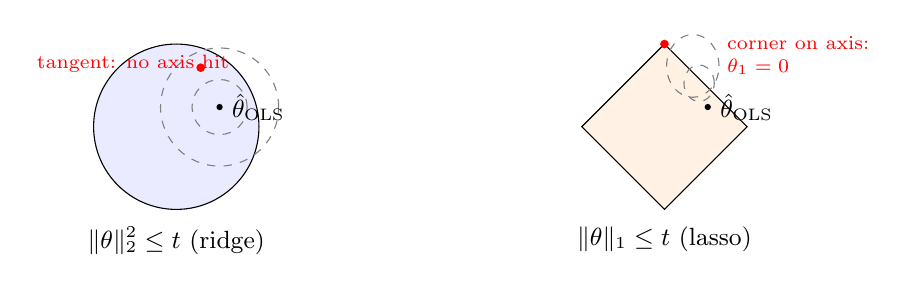
\begin{tikzpicture}[font=\small]
  % L2 ball
  \begin{scope}[shift={(0,0)}]
    \fill[blue!8] (0,0) circle (1.05);
    \draw (0,0) circle (1.05);
    \node[below] at (0,-1.15) {$\|\theta\|_2^2 \le t$ (ridge)};
    \foreach \r in {0.35,0.75} \draw[dashed, gray] (0.55,0.25) circle (\r);
    \fill (0.55,0.25) circle (0.04) node[right=1pt] {$\hat\theta_{\rm OLS}$};
    \fill[red] (0.31,0.75) circle (0.055);
    \node[red, font=\scriptsize] at (-0.55,0.8) {tangent: no axis hit};
  \end{scope}
  % L1 ball
  \begin{scope}[shift={(6.2,0)}]
    \fill[orange!10] (0,1.05) -- (1.05,0) -- (0,-1.05) -- (-1.05,0) -- cycle;
    \draw (0,1.05) -- (1.05,0) -- (0,-1.05) -- (-1.05,0) -- cycle;
    \node[below] at (0,-1.15) {$\|\theta\|_1 \le t$ (lasso)};
    \foreach \s in {0.55,0.95}
      \draw[dashed, gray] ({0.55-0.2*\s},{0.25+0.55*\s}) ellipse ({0.35*\s} and {0.42*\s});
    \fill (0.55,0.25) circle (0.04) node[right=1pt] {$\hat\theta_{\rm OLS}$};
    \fill[red] (0,1.05) circle (0.055);
    \node[red, font=\scriptsize, align=left] at (1.7,0.9) {corner on axis:\\$\theta_1 = 0$};
  \end{scope}
\end{tikzpicture}
\caption{Why lasso gives zeros. The constraint region (filled) grows until
it kisses the loss contours (dashed). The smooth circle can touch anywhere;
the diamond's corners sit on the axes, so the first touch is usually a
corner --- some coefficient \emph{exactly} zero.}\label{fig:geometry}
\end{figure}

\lstinputlisting[language=Python,caption={\texttt{code/ch04/reg\_compare.py}: scratch-grade comparison --- OLS, ridge, lasso on \texttt{diabetes}, then the lasso kill-order on \texttt{california}.},label={lst:regcmp}]{code/ch04/reg_compare.py}

\lstinputlisting[numbers=none]{code/ch04/reg_compare.out.txt}

\begin{example}[WE 4.2 --- Reading the kill order]\label{ex:killorder}
Strategy: which feature dies first under $\ell_1$ is the feature the data
voted least useful.\par
\begin{solution}
On \texttt{diabetes}, lasso at $\alpha{=}0.05$ already zeros \texttt{s2}
($-0.00$) and shrinks the blood-serum cluster hard --- the six serum
measurements largely repeat each other's information, and lasso picks a
spokesperson (\texttt{s5} keeps $536.93$). On \texttt{california},
\texttt{Population} dies first (gone by $\alpha{=}0.01$), and at
$\alpha{=}0.1$ only \texttt{MedInc}, \texttt{HouseAge}, and
\texttt{Latitude} survive --- income dominates California housing prices,
a claim lasso states as an absence rather than a coefficient. Test $R^2$
actually \emph{improves} ($0.404 \to 0.422$): the deleted features were
costing variance.
\end{solution}
\end{example}

\begin{figure}[ht]\centering
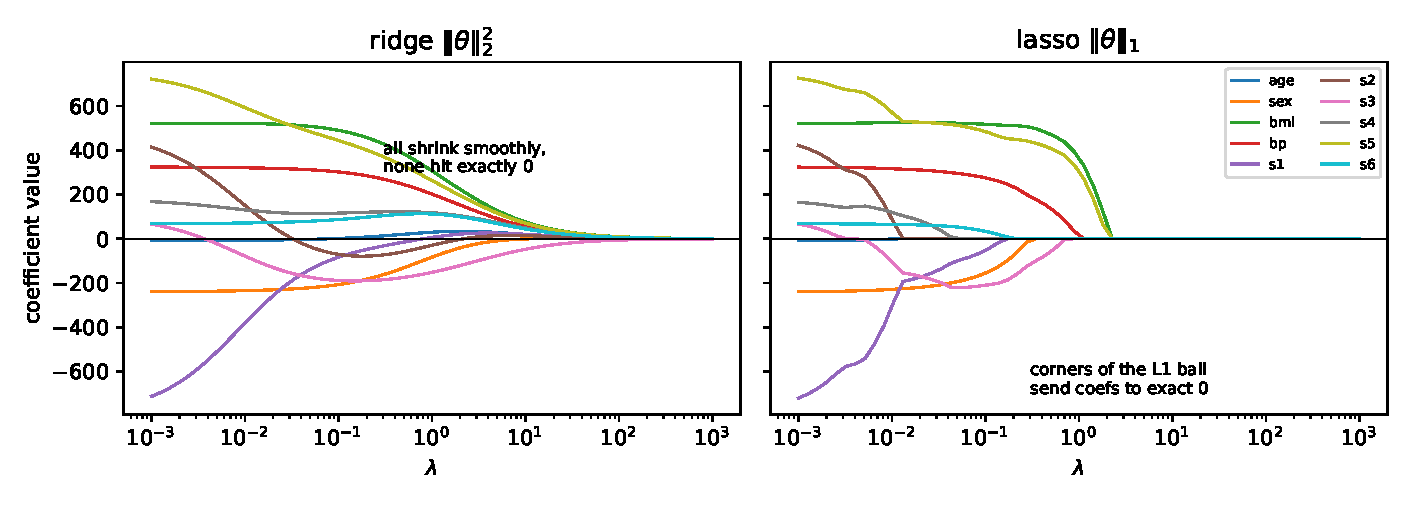
\includegraphics[width=\linewidth]{figures/ch04/coef_paths.pdf}
\caption{Coefficient paths vs $\lambda$ on \texttt{diabetes}
(\texttt{figures/fig\_ch04\_coef\_paths.py}). Ridge shrinks all ten
coefficients smoothly toward zero; lasso's path is piecewise linear and
each kink is a feature dying --- the geometric difference of
Figure~\ref{fig:geometry} plotted.}\label{fig:paths}
\end{figure}

\section{Logistic regression: regression for labels}\label{sec:logreg}

For classification, regress the \emph{log-odds} instead of the label. The
sigmoid\index{sigmoid} squashes the linear score into a probability:
\[
p = \sigma(\mathbf{w}^T\mathbf{x} + b), \qquad
\sigma(z) = \frac{1}{1 + e^{-z}}.
\]
Training minimises the negative log-likelihood (a.k.a.\ cross-entropy
loss\index{cross-entropy}), which has no closed-form minimum but a clean
gradient ---
$\nabla_{\mathbf w}\mathrm{NLL} = \frac{1}{n}X^T(\mathbf{p} - \mathbf{y})$
--- so gradient descent does the fitting. Listing~\ref{lst:logreg}
implements it in a dozen lines; the loss trace (NLL $261 \to 93$) is the
descent working.

\lstinputlisting[language=Python,caption={\texttt{code/ch04/logreg\_scratch.py}: logistic regression by gradient descent, NLL computed with the numerically stable \texttt{logaddexp}.},label={lst:logreg}]{code/ch04/logreg_scratch.py}

\lstinputlisting[numbers=none]{code/ch04/logreg_scratch.out.txt}

\begin{example}[WE 4.3 --- Read the weights as a story]\label{ex:weights}
Strategy: a fitted coefficient is a claim about a feature, in odds.
\par
\begin{solution}
On the two strongest \texttt{breast\_cancer} features the model learns
$\mathbf{w} = (-6.86,\ 0.61)$: a unit rise in standardised \emph{worst
radius} swings the log-odds $-6.86$ toward malignant --- huge, because
radius is nearly diagnostic by itself. Test accuracy $0.930$, precision
$0.957$, recall $0.931$: $6$ of $114$ wrong, and the errors are the
borderline-radius patients the sigmoid honestly scored near $0.5$. A
linear boundary doing $93\%$ is why this dataset is the canonical warm-up.
\end{solution}
\end{example}

\begin{figure}[ht]\centering
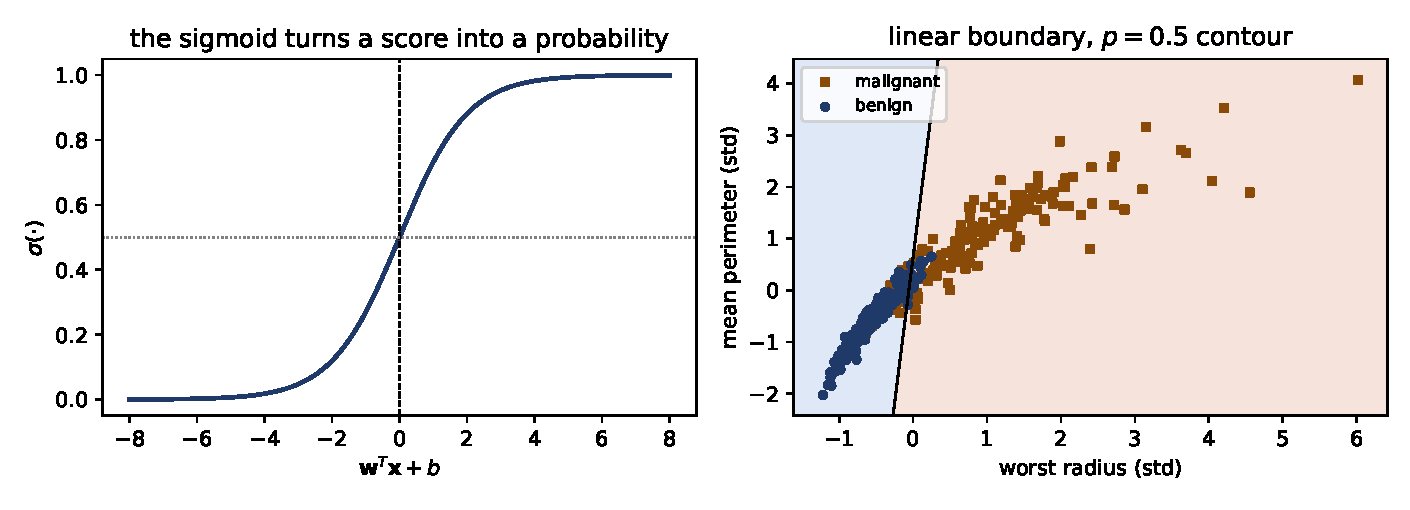
\includegraphics[width=\linewidth]{figures/ch04/sigmoid_boundary.pdf}
\caption{Left: the sigmoid. Right: the learned $p{=}0.5$ boundary on two
standardised features (\texttt{figures/fig\_ch04\_sigmoid\_boundary.py})
--- a straight line in feature space, because the model is linear in
$\mathbf{x}$ whatever the sigmoid does to its output.}\label{fig:sigmoid}
\end{figure}

\section{Softmax: one boundary, many classes}\label{sec:softmax}

Multiclass generalises pairwise: one weight vector per class, scores
$\mathbf{z} = W\mathbf{x}$, and the softmax\index{softmax}
\[
P(y{=}c \mid \mathbf{x}) = \frac{e^{z_c}}{\sum_j e^{z_j}}
\]
normalises them into a distribution. Training minimises cross-entropy on
the true class's probability --- the same NLL with more terms. Nothing new
to learn mathematically; the lesson is that ``multinomial logistic
regression'' is just logistic regression with a softmax head, and every
classifier in the deep-learning chapters ends this way.

\section{Feature maps: bend the input, keep the line}\label{sec:featmaps}

Linear in $\mathbf{x}$ need not mean linear in \emph{appearance}: fit
$\mathbf{w}^T\phi(\mathbf{x})$ where
$\phi(x) = (1, x, x^2, \dots, x^p)$ and the model is a degree-$p$
polynomial\index{feature map} while still linear in $\boldsymbol\theta$
--- OLS machinery applies verbatim. The cost is expressivity's usual price:
Figure~\ref{fig:polyfit} shows degree-9 threading every data point while
oscillating wildly between them --- $R^2 = 1.00$ on train, hopeless on
test.

\begin{figure}[ht]\centering
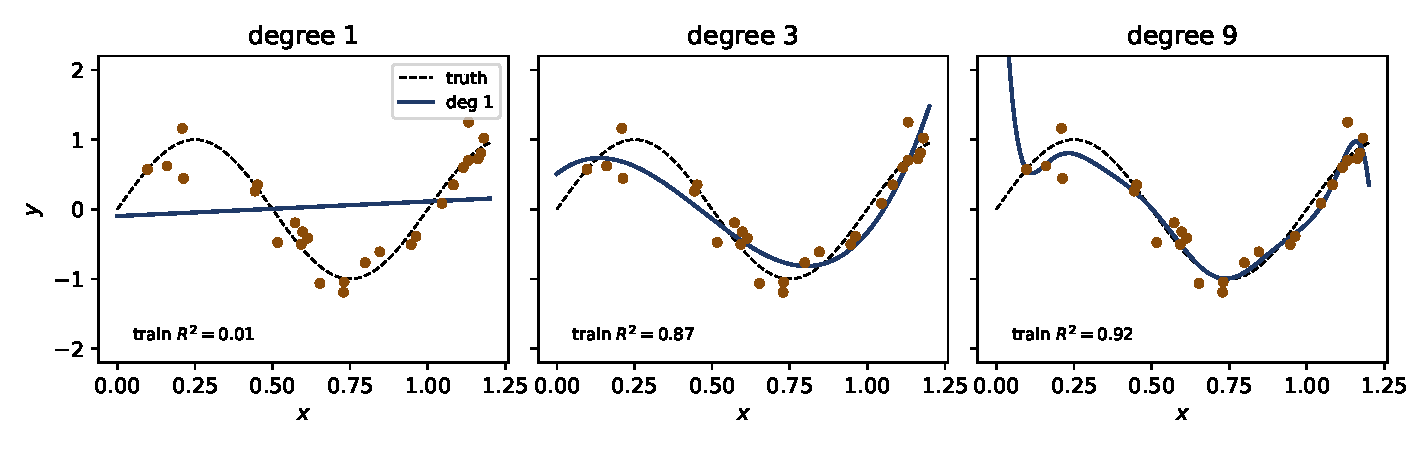
\includegraphics[width=\linewidth]{figures/ch04/poly_overfit.pdf}
\caption{Polynomial degrees 1, 3, 9 on the same 26 points
(\texttt{figures/fig\_ch04\_poly\_overfit.py}). Degree 3 approximates the
truth; degree 9 memorises it --- the overfit strip is the visual version
of the $\lambda \to 0$ end of the U-curve.}\label{fig:polyfit}
\end{figure}

\section{The kernel trick in one page}\label{sec:kernel}

Every algorithm in this chapter touches data only through inner products
$\mathbf{x}_i^T\mathbf{x}_j$. Replace each with a kernel
$K(\mathbf{x}_i,\mathbf{x}_j) = \phi(\mathbf{x}_i)^T\phi(\mathbf{x}_j)$
and you fit in the $\phi$-space \emph{without ever computing $\phi$} ---
even infinite-dimensional ones (the RBF kernel). SVMs are the maximally
squeezed version of this idea: maximum-margin hyperplane plus kernel.
We will not implement one --- the point to carry forward is that
``linear model'' and ``nonlinear model'' differ only in the features you
let the dot product see.\index{kernel trick}

\section{Common mistakes}

\begin{description}
\item[Penalising the intercept] The bias term absorbs the mean of
  $\mathbf{y}$; shrinking it toward zero is a bug in most setups. Sklearn
  and Listing~\ref{lst:linreg} both exempt it --- mimic that.
\item[Regularising unscaled features] A penalty treats all coefficients
  equally only if all features share a scale. Standardise before
  ridge/lasso or the biggest-unit column gets punished hardest.
\item[Choosing $\lambda$ on the test set] $\lambda$ is a hyperparameter:
  pick it by CV inside training, then touch test once (Chapter 3's
  protocol, verbatim).
\item[Reading lasso zeros as ``feature is useless''] Correlated features
  split the vote --- lasso keeps a spokesperson, not a ranking. The
  survivors are useful; the dead are only redundant-or-useless.
\item[Forming $(X^TX)^{-1}$ explicitly] \texttt{np.linalg.solve} is
  faster and far more stable than \texttt{inv}; the inverse you never
  form cannot amplify your conditioning error.
\item[Assuming ``linear'' means a line] Polynomial maps, interactions,
  basis expansions --- the model is linear in $\boldsymbol\theta$, and
  that is the only linearity that matters.
\item[Forgetting sigmoid probabilities need calibration] $\sigma(z)$ is
  a score shaped like a probability; whether it \emph{is} one depends on
  calibration (Platt scaling, isotonic) --- check before quoting odds.
\item[Using MSE for classification] Cross-entropy is the MLE loss for
  Bernoulli labels; least-squares on 0/1 targets works accidentally and
  optimises the wrong thing.
\item[Blind trust in $R^2$ on test] A high test $R^2$ after fitting
  preprocessing on all data is Chapter 3's leak in a trench coat ---
  refit the pipeline inside the split.
\end{description}

\section{Summary table}

\begin{tabularx}{\linewidth}{@{}l l X@{}}
\toprule
\textbf{Model} & \textbf{Objective} & \textbf{When to reach for it}\\
\midrule
OLS & $\|X\theta - y\|^2$ & baseline regression; full rank, low $d$\\
Ridge & $\;+\lambda\|\theta\|_2^2$ & correlated features; wants stability\\
Lasso & $\;+\lambda\|\theta\|_1$ & feature selection by zeros; sparse truth\\
Elastic net & $\;+\lambda_1\|\theta\|_1 + \lambda_2\|\theta\|_2^2$ &
  correlated \emph{and} sparse\\
Logistic & cross-entropy on $\sigma(w^Tx)$ & binary probabilities, fast\\
Softmax & cross-entropy on $\mathrm{softmax}(Wx)$ & multiclass one-liner\\
Poly.~map & $\phi(x)$ inside OLS & smooth nonlinear, small $n$\\
Kernel & $K(x_i, x_j)$ inner products & nonlinear at linear-model cost\\
\bottomrule
\end{tabularx}

\section{Drill --- five concept questions}

\begin{enumerate}
\item Ridge and lasso differ by one letter of subscript. What do the
  resulting coefficient paths look like, and why?
\item Why does the test MSE form a U in $\lambda$ while train MSE is
  monotone?
\item $X^TX$ is singular. Name the regulariser whose solution still
  exists, and what it picks out of the infinite OLS family.
\item Logistic regression minimises NLL, not MSE --- what does NLL
  correspond to probabilistically?
\item Degree-9 polynomial scores train $R^2 = 1.00$. Bias problem or
  variance problem, and which chapter-3 diagnostic confirms it?
\end{enumerate}

\section*{Further reading}
\begin{itemize}
\item Hastie, Tibshirani \& Friedman --- \emph{The Elements of
  Statistical Learning}. \url{https://hastie.su.domains/ElemStatLearn/}
  --- ch.~3 is the canonical ridge/lasso treatment behind
  Figure~\ref{fig:geometry}.
\item Hastie, Tibshirani \& Wainwright --- \emph{Statistical Learning
  with Sparsity} (book site; free PDF). \url{https://hastie.su.domains/StatLearnSparsity/}
  --- the $\ell_1$ book; ch.~1--3 cover lasso geometry and paths.
\item scikit-learn --- \emph{Linear models} user guide.
  \url{https://scikit-learn.org/stable/modules/linear_model.html} ---
  \texttt{Ridge}/\texttt{Lasso}/\texttt{LogisticRegression} parameters as
  used in the listings.
\item James, Witten, Hastie \& Tibshirani --- \emph{An Introduction to
  Statistical Learning} (free PDF). \url{https://www.statlearning.com/}
  --- the gentler ESL; ch.~4 classification and ch.~6 regularisation.
\item Ng, Andrew --- \emph{CS229 Lecture Notes 1}.
  \url{https://see.stanford.edu/materials/aimlcs229/cs229-notes1.pdf} ---
  normal equations and logistic regression derived slowly, by hand.
\item Molnar --- \emph{Interpretable Machine Learning}, linear models
  chapter. \url{https://christophm.github.io/interpretable-ml-book/limo.html}
  --- reading coefficients responsibly, incl.\ the correlated-features
  caveat from WE~4.2.
\item Wikipedia --- ``Lasso (statistics)''.
  \url{https://en.wikipedia.org/wiki/Lasso_(statistics)} --- quick
  formulas, history (Tibshirani 1996), and the geometric figure this
  chapter redrew.
\end{itemize}

\begin{rulebox}{Watch instead (if you'd rather see it)}
\begin{itemize}
\item \textbf{StatQuest: Regularization Part 1 --- Ridge (L2)
  Regression} (20:26). StatQuest with Josh Starmer.
  \url{https://www.youtube.com/watch?v=Q81RR3yKn30} --- ridge as
  ``desensitisation,'' matching \S\ref{sec:ridge}; includes the
  unsolvable-problem story of WE~4.1. Accessed 2026-10-11.
\item \textbf{StatQuest: Regularization Part 2 --- Lasso (L1)
  Regression} (8:19). StatQuest with Josh Starmer.
  \url{https://www.youtube.com/watch?v=NGf0voTMlcs} --- the contrast half
  of the pair; matches \S\ref{sec:lasso}. Accessed 2026-10-11.
\item \textbf{StatQuest: Logistic Regression} (8:47). StatQuest with Josh
  Starmer. \url{https://www.youtube.com/watch?v=yIYKR4sgzI8} --- sigmoid
  and likelihood behind \S\ref{sec:logreg}. Accessed 2026-10-11.
\end{itemize}
\end{rulebox}

\chapternotes
\begin{enumerate}
\item The normal equations are fine for $d$ up to a few thousand; beyond
  that, QR or SVD is stabler, and at scale the gradient methods of
  \S\ref{sec:logreg} take over entirely (Hastie et al.\ ch.~3
  \cite{hastie2009}).
\item Lasso is Tibshirani (1996), ridge is Hoerl \& Kennard (1970) ---
  invented precisely for WE~4.1's singular case, decades before ``ML''
  was a word for it.
\item The elastic net mixes both penalties and inherits both behaviours;
  it is the default answer when correlated features are also sparse
  (Zou \& Hastie 2005).
\item Cross-entropy is negative log-likelihood under the Bernoulli model
  --- the same quantity computed two ways. The gradient
  $X^T(\mathbf p - \mathbf y)/n$ is derived fully in Ng's notes (Further
  reading).
\item We skipped kernel details on purpose; Cawley \& Talbot
  \cite{cawley2010} (ch.~3's list) is again the citation for how
  hyperparameter choice corrupts honest evaluation.
\end{enumerate}

\section*{Exercises}

\emph{[easy]}
\begin{exercise}
Write the normal equations from the residual-orthogonality argument in
one line each: (a) the residual, (b) the orthogonality, (c) the solution.
\end{exercise}
\begin{exercise}
In Listing~\ref{lst:linreg}, which $\lambda$ minimises test MSE, and
what is $\|\boldsymbol\theta\|$ there? Why does $\|\theta\|$ fall
monotonically?
\end{exercise}
\begin{exercise}
On \texttt{california}, which feature dies first under lasso and which
survives longest? One sentence of economic intuition.
\end{exercise}
\begin{exercise}
Why does logistic regression output $\sigma(\mathbf w^T \mathbf x)$
rather than $\mathbf w^T \mathbf x$ itself? What breaks if you skip the
sigmoid?
\end{exercise}

\emph{[medium]}
\begin{exercise}
Implement \texttt{ridge\_fit(X, y, lam)} with an unpenalised intercept,
and verify your coefficients match \texttt{Ridge(alpha=lam)} up to
$10^{-6}$.
\end{exercise}
\begin{exercise}
Sweep the logistic decision threshold on the WE~4.3 model; find the
threshold maximising $F_1$ and the threshold giving recall $\ge 0.98$.
Which would a screening program pick?
\end{exercise}
\begin{exercise}
Implement a 2-fold CV selector for lasso's $\alpha$ on
\texttt{diabetes}; report the $\alpha$ that minimises CV MSE and its
test $R^2$.
\end{exercise}
\begin{exercise}
Fit degree-3 polynomial on the Figure~\ref{fig:polyfit} data with
ridge $\lambda=1$ and without it; measure the test MSE gap regularisation
buys at fixed degree.
\end{exercise}
\begin{exercise}
Reproduce Figure~\ref{fig:paths}'s lasso panel with
\texttt{linear\_model.lars\_path} and confirm the kink positions match
the coefficient-zero crossings.
\end{exercise}
\begin{exercise}
Elastic net from scratch: implement coordinate descent for the
$\ell_1{+}\ell_2$ objective on \texttt{diabetes} and compare the survivor
set to pure lasso.
\end{exercise}

\emph{[hard]}
\begin{exercise}
Derive $\nabla_{\mathbf w}\mathrm{NLL} = \frac{1}{n}X^T(\mathbf p -
\mathbf y)$ for the logistic model, starting from the Bernoulli
likelihood. (This is the one derivation every interview asks.)
\end{exercise}
\begin{exercise}
Prove the ridge solution exists and is unique for every $\lambda > 0$
even when $X^TX$ is singular --- i.e.\ $X^TX + \lambda I \succ 0$.
\end{exercise}
\begin{exercise}
Show the lasso soft-threshold rule: in 1-D, the coordinate-wise solution
is $\mathrm{sign}(z)\max(|z| - \lambda, 0)$; explain geometrically why
this produces exact zeros.
\end{exercise}
\begin{exercise}
Design the singular-rescue experiment quantitatively: on WE~4.1's
redundant design, plot $\|\boldsymbol\theta\|$ vs $\lambda$ from
$10^{-6}$ to $10^{3}$ and locate where the cancellation disappears.
\end{exercise}
\begin{exercise}
Prove logistic regression's decision boundary is linear, then show the
\emph{probability} contours are also linear --- the sigmoid bends the
numbers, never the geometry.
\end{exercise}

\section*{Hints and answers}
\begin{description}
\item[4.1] $X^TX\theta = X^Ty$ follows from $X^T(X\theta - y) = 0$.
\item[4.2] $\lambda \approx 0.1$ gives MSE $2861$; the penalty pulls all
  coefficients toward the origin at once.
\item[4.3] \texttt{Population} first, \texttt{MedInc} last --- income is
  the strongest single driver of California house price.
\item[4.4] Probabilities need $[0,1]$; raw scores ignore boundedness and
  calibration.
\item[4.5] Solve without inverting: standardise, append the ones column,
  then \texttt{solve} --- match sklearn's intercept separately.
\item[4.6] High recall needs a low threshold; screening pays for
  precision later.
\item[4.7] 2-fold is enough to rank $\alpha$'s; expect $\alpha \approx
  0.01$--$0.1$ to win.
\item[4.8] Ridge at degree 3 barely changes the fit; its value shows up
  at degree 9 --- try both.
\item[4.9] \texttt{lars\_path} returns the exact knot grid; the kinks are
  where a coefficient enters or leaves the active set.
\item[4.10] Coordinate descent loops one coordinate at a time with the
  soft threshold of 4.13.
\item[4.11] Write $L = \prod p_i^{y_i}(1-p_i)^{1-y_i}$, take
  $-\log$, differentiate --- the derivative of $\sigma$ factorises
  beautifully.
\item[4.12] Any $v \neq 0$: $v^T(X^TX)v = \|Xv\|^2 \ge 0$, plus
  $\lambda v^Tv > 0$.
\item[4.13] The kink at $|z| = \lambda$ is the $\ell_1$ corner in
  miniature; below it the subgradient contains zero and the optimum
  \emph{is} zero.
\item[4.14] Plot should show $\|\theta\|$ collapsing around
  $\lambda \sim 10^{-2}$--$10^{-1}$ as the cancelling pair joins the
  shrunk family.
\item[4.15] $\mathbf{w}^T\mathbf{x} + b = c$ is a hyperplane for every
  $c$; $\sigma$ is monotone, so level sets coincide.
\end{description}
